% IMPORTANT: PLEASE USE XeLaTeX FOR TYPESETTING
\documentclass{sintefbeamer}
\usepackage{xeCJK}
\usepackage{amsthm}
\setbeamertemplate{theorems}[numbered]
\makeatletter
\setbeamertemplate{footline}
{
  \leavevmode%
  \hbox{%
  \begin{beamercolorbox}[wd=.7\paperwidth,ht=2.25ex,dp=1ex,center]{title in head/foot}%
    \usebeamerfont{title in head/foot} {GFL: Federated Learning on Non-IID data via Privacy-preserving Synthetic data}
  \end{beamercolorbox}%
  \begin{beamercolorbox}[wd=.3\paperwidth,ht=2.25ex,dp=1ex,right]{date in head/foot}%
    \usebeamerfont{date in head/foot}\insertshortdate{}\hspace*{2em}
    \insertframenumber{} / \inserttotalframenumber\hspace*{2ex} 
  \end{beamercolorbox}}%
  \vskip0pt%
}

%\newtheorem{theorem}{Theorem} % to number according to section
\theoremstyle{definition}

\makeatother

% meta-data
\title{\huge GFL: Federated Learning on Non-IID Data via Privacy-preserving Synthetic Data}
\subtitle{汇报人:黄其涵 \qquad 导师:章静 教授 \qquad }
\author{2023 IEEE International Conference on Pervasive Computing and Communications (PerCom)}
\date{\today}
\titlebackground{images/bg4}

% document body
\begin{document}

\maketitle


\section{研究背景}

\begin{frame}{1.1 联邦学习}
\begin{itemize}
\item 联邦学习是一种分布式机器学习方法,其利用一个中央服务器(也称为服务器端)协调各终端设备(也称为客户端),协同训练一个各客户端共享的全局模型。

\item 与传统中心化训练方法不同,\textbf{联邦学习不需要各设备发送自身隐私数据至数据中心,因此有利于保护数据隐私。}具体而言,联邦学习在客户端和服务器端之间通过多轮通信迭代优化模型。
\item 每轮通信包含两个阶段:
\begin{itemize}
\item[(1)]各客户端从服务器端下载全局模型,并在本地数据上进行训练以获得本地模型;
\item[(2)]服务器端接收并聚合各客户端的本地模型参数以获得性能更优的全局模型.然而,现有联邦学习机制尚面临两大不足。
\end{itemize}
\end{itemize}

\end{frame}

\begin{frame}{1.1 联邦学习}
\begin{itemize}
\item 联邦学习是一种分布式机器学习方法,其利用一个中央服务器(也称为服务器端)协调各终端设备(也称为客户端),协同训练一个各客户端共享的全局模型。

\item 与传统中心化训练方法不同,\textbf{联邦学习不需要各设备发送自身隐私数据至数据中心,因此有利于保护数据隐私。}具体而言,联邦学习在客户端和服务器端之间通过多轮通信迭代优化模型。
\item 每轮通信包含两个阶段:
\begin{itemize}
\item[(1)]各客户端从服务器端下载全局模型,并在本地数据上进行训练以获得本地模型;
\item[(2)]服务器端接收并聚合各客户端的本地模型参数以获得性能更优的全局模型.然而,现有联邦学习机制尚面临两大不足。
\end{itemize}
\end{itemize}

\end{frame}

\begin{frame}{1.2 现有问题}
\begin{columns}
\begin{column}{0.45\textwidth}
\begin{figure}[ht]
\centering
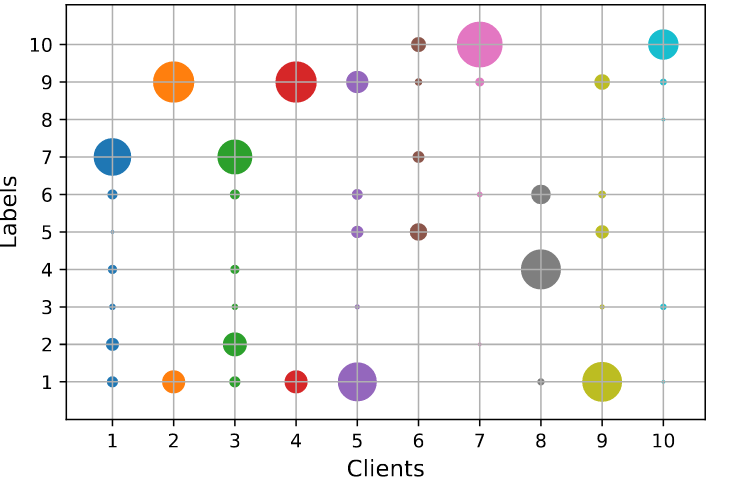
\includegraphics[width=1\textwidth]{images/img_unbalance}
\end{figure}
\end{column}
\begin{column}{0.65\textwidth}
\begin{itemize}
\item \textbf{类别不均衡。}全局模型需考虑多个客户端的数据,但各客户端往往仅包含部分类别数据且类别间数据量严重不均衡,使得全局模型难以训练。所训练的本地模型容易过拟合本地数据而在全局数据上往往取得较差性能。更重要的是,这些性能较差的本地模型严重影响全局模型的训练,导致难以构建高性能全局模型。
\item \textbf{数据分布差异。}由于各客户端的功能和用户使用习惯不同,不同客户端往往产生不同类别的数据,导致各客户端数据之间的类别分布差异较大。
\end{itemize}
\end{column}
\end{columns}
\end{frame}


\begin{frame}{1.3 主要贡献}
\begin{itemize}
\item \textbf{本文提出基于GAN的GFL框架以解决FL中数据异构性问题,并为 FL 系统构建高性能全局模型。 }GFL 促进了 FL 训练过程,同时保持了成员身份的隐私和原始数据在客户中的分布。
\item \textbf{本文提出了一种保护隐私的数据生成工作流程,以生成符合我们隐私设置的合成样本。} DPGAN 用于生成满足差分隐私的样本,以保护客户端免受成员推理攻击。本文生成大量合成数据并选择一个随机分布的子集来隐藏客户端的真实数据分布。
\item \textbf{本文对合成数据进行“iidify”处理,以 iid 方式训练全局模型,并使用 Epoch Decay 参数来解决模式崩溃问题并避免使用低质量的合成数据。}
\end{itemize}
\end{frame}

\section{问题定义}

\begin{frame}{2 优化目标}

\begin{columns}
\begin{column}{0.4\textwidth}
\begin{figure}[ht]
\centering
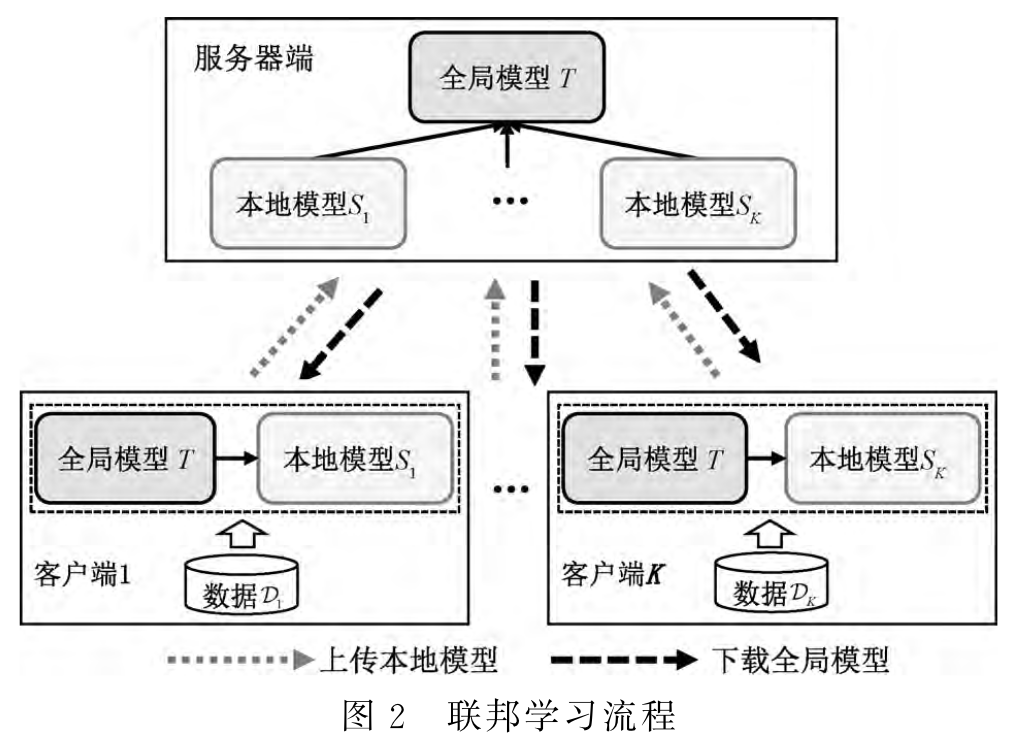
\includegraphics[width=1\textwidth]{images/img_fl}
\end{figure}
\end{column}
\begin{column}{0.6\textwidth}
为解决上述难题, 本文提出在客户端构造类别均衡的数据集进行训练的策略。 令 $\mathcal{D}$ 表示所构造的类别 均衡数 据集, $M$ 表示全局数据的类别数,则 
$$
\mathcal{D}=\left\{(x, y) \mid P(y=i)=\frac{1}{M}, \quad i \in\{0,1, \ldots, M-1\}\right\}
$$
其中 $p(\mathcal{D})$ 表示数据集 $\mathcal{D}$ 所代表的经验分布. 因此, 本文 旨在解决如下优化问题:
$$
\min _{\boldsymbol{W}_T} \mathbb{E}_k\left[\mathbb{E}_{x_k \sim p(\mathcal{D})}\left[\mathcal{L}\left(x_k ; \boldsymbol{W}_T\right)\right]\right]
$$
与仅仅利用客户端本地数据进行训练的方式相比,基于类别均衡的数据集进行训练使得各客户端本地模型之间的差异大大减少。
\end{column}
\end{columns}


\end{frame}

\section{研究方法}

\begin{frame}{3.1  Overview of Generative Federated Learning (GFL)}
\centering
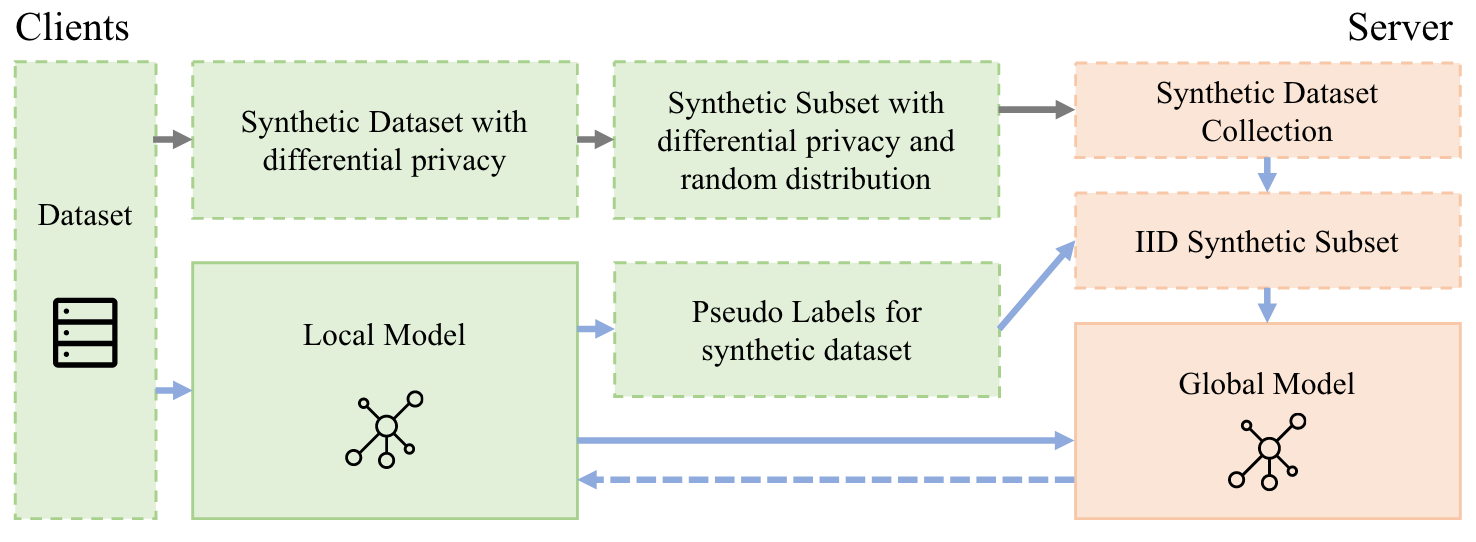
\includegraphics[width=1\textwidth]{images/gfl_overview}

\end{frame}

	


\begin{frame}{3.2 Synthetic Data Generation}


\begin{columns}
\begin{column}{0.5\textwidth}
\begin{figure}[ht]
\centering
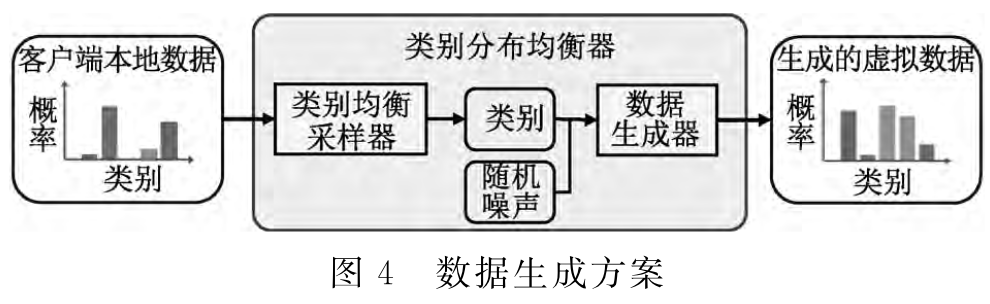
\includegraphics[width=1\textwidth]{images/img_gan}
\end{figure}

类别均衡采样器构造完成后, 各客户端根据采 样概率 $\widetilde{P}_m$ 采样相应的类别 $m$。 值得注意的是, 该过程在客户端进行, 客户端的数据分布信息不会发送至服务器端。
\end{column}
\begin{column}{0.5\textwidth}
(1) 统计客户端上类别 $m$ 的概率:
$$
P_m=\frac{n_m}{\sum_{m=0}^{M-1} n_m}
$$
(2)计算与客户端上类别分布相反的采样概率, 即类别 $m$ 的采样概率为:
$$
\bar{P}_m=1-P_m
$$
(3) 归一化采样概率:
$$
\widetilde{P}_m=\frac{\bar{P}_m}{\sum_{m=0}^{M-1} \bar{P}_m}
$$
\end{column}
\end{columns}


\end{frame}


\begin{frame}{3.3 Federated Learning with Synthetic Data}{数据生成器}
通过类别均衡采样器, 客户端可获得各类别的 采样量。 然而, 如何根据所采样的类别获得相应的 数据以用于本地模型的训练仍然是一个难题。 为解 决该问题, 本文引入了数据生成器 $G$。\textbf{该数据生成 器的输人为类别标签 $y$ 和噪声矢量 $z$。 其中 $y \in$ $\{0,1, \ldots, M-1\}, z$ 服从高斯分布 $N(0,1)$。}  数据生 成器 $G$ 根据噪声矢量 $z$ 和类别标签 $y$ 生成相应的数据 $\hat{x}$, 即
$$
\hat{x}=G(z \mid y), z \sim N(0,1) 
$$
数据生成器和类别均衡采样器构造完成后, 客户端首先根据类别均衡采样器采样类别 $m$, 然后利用数据 生成器生成类别为 $m$ 的虚拟数据。 最后, 客户端结 合本地数据和生成的虚拟数据, 从而构造类别均衡 的数据集来训练本地模型。
\end{frame}





\section{实验分析}

\begin{frame}{4.1 数据集}
在我们的实验中,我们使用 DPGAN 作为Local GAN模型,ResNet18 作为 EMNIST 和 CIFAR-10联邦学习的训练模型。

	\begin{itemize}
\item[1)] EMNIST。 在实验中使用它的“Digits”子集。它包含 10 个类,总共 280, 000 个样本,分为 240, 000 个训练样本和 40, 000 个测试样本。与 MNIST 相比,它拥有更多数据并且完全平衡。
\item[2)] CIFAR-10。它包含 10 个不同类别的 60, 000 个 32 × 32 彩色图像,与 EMNIST 相比,这是一项更复杂的任务。我们使用这个数据集来衡量 GFL 在艰巨任务中的稳定性。
\end{itemize}
\end{frame}

\begin{frame}{4.2 对比模型}
本文将GFL与目前最新的方法进行比较,即FedAvg、FedPoxr、SCAFFOLD和FedNvao.本实验通过狄利克雷分布Dir(0.1)模拟各客户端数据的类别分布.所有方法基于两种常见的深度神经网络模型(即ResNet20和MobileNet V2)进行训练和性能比较。
	\\ \hspace*{\fill} \\
GFL 在合成数据生成阶段训练了 200 个 epoch。然后,我们从每个客户端 $k$ 中随机选择 $n_{S_k}=500$  个合成样本。在联邦学习阶段,初始全局训练 epoch $E_s$ 设置为 10,如果未指定,epoch decay 参数 $\tau$ 设置为 0.1。
	\\ \hspace*{\fill} \\
上述所有算法共享相同的基本训练设置。训练包含 100 轮通信,每轮每个客户端训练 20 个 epoch,服务器和客户端的批大小都设置为 128。
\end{frame}


\begin{frame}{4.3 实验结果}{Result Analysis}
	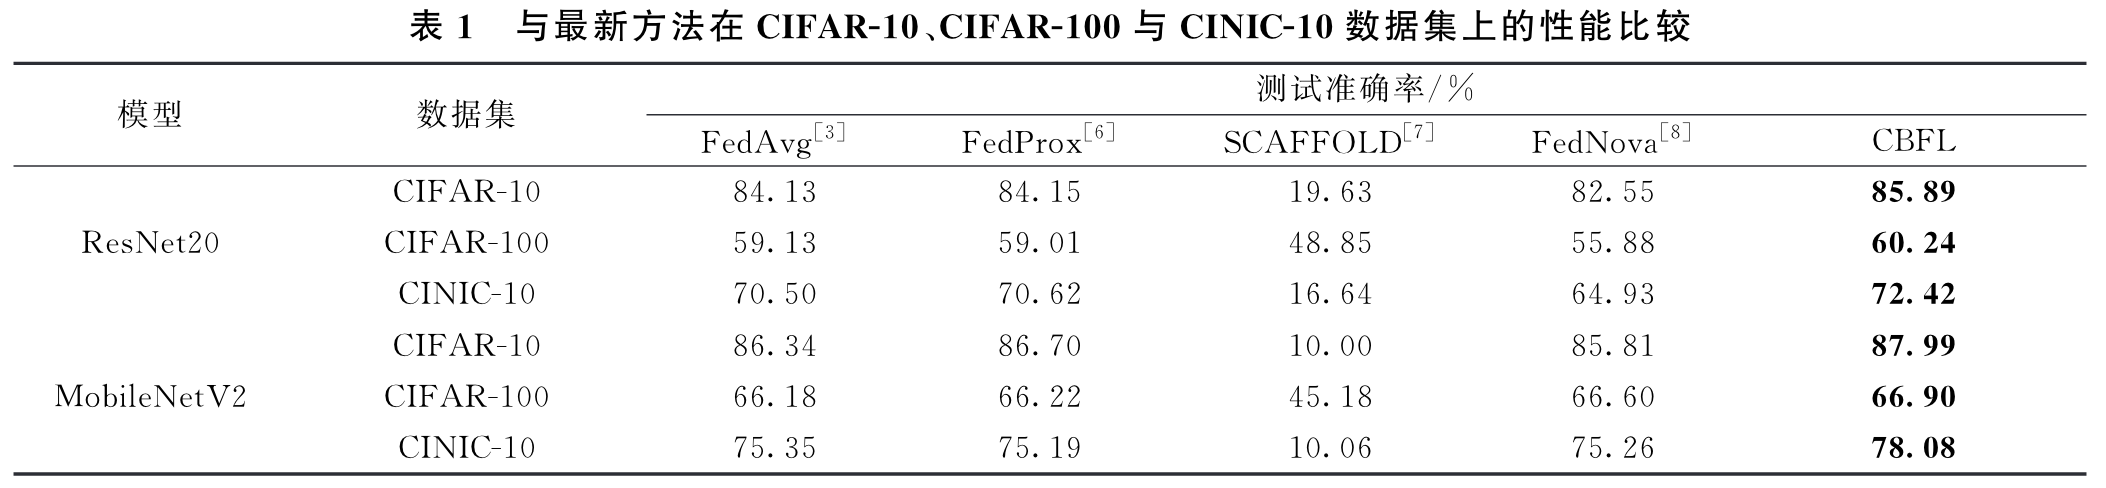
\includegraphics[width=1.\textwidth]{images/img_expr2}
\end{frame}

\begin{frame}{4.3 实验结果}{Result Analysis}
	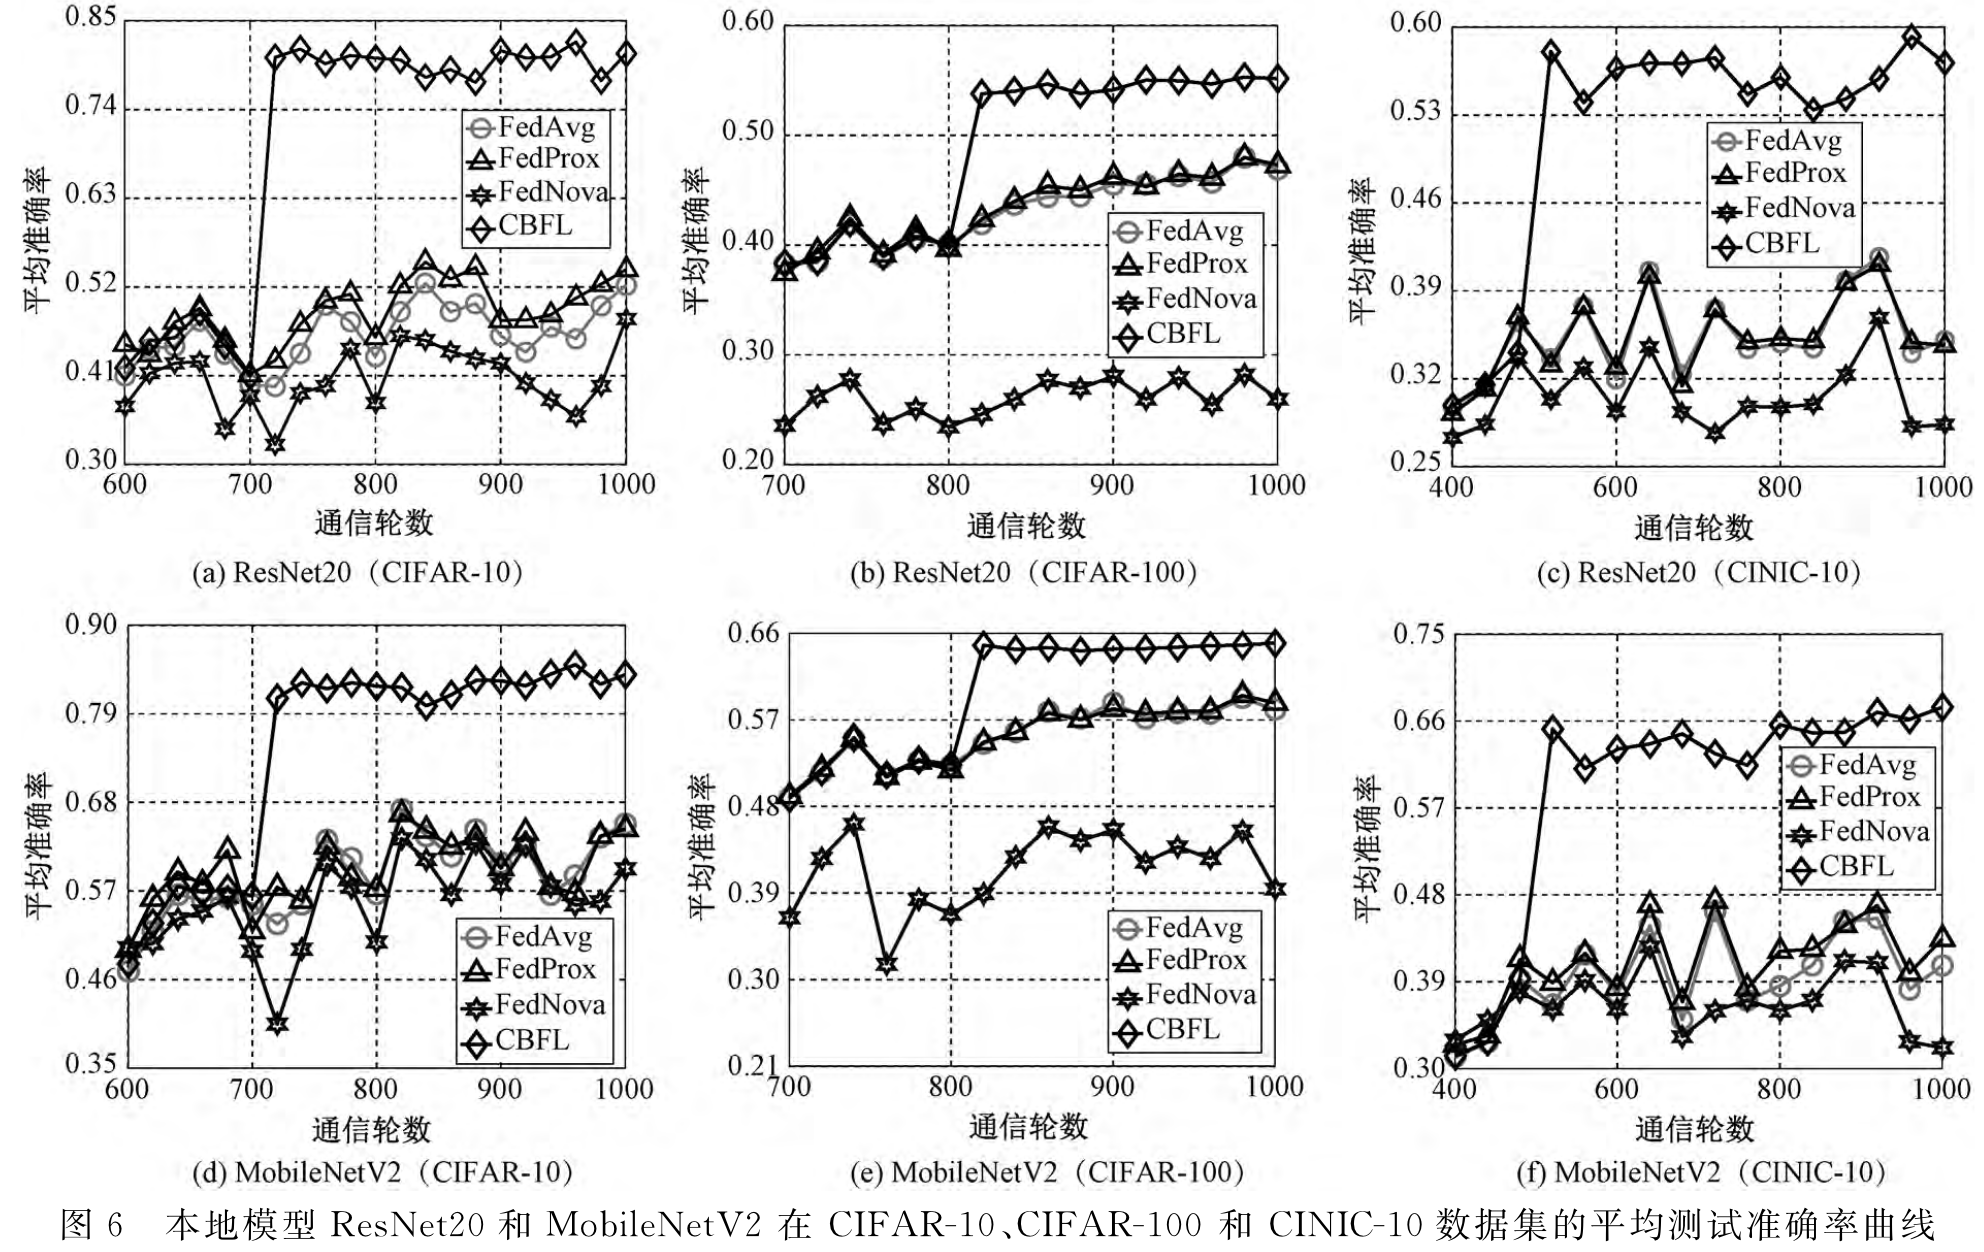
\includegraphics[width=0.75\textwidth]{images/img_expr1}
\end{frame}

\begin{frame}{4.3 实验结果}{Result Analysis}
	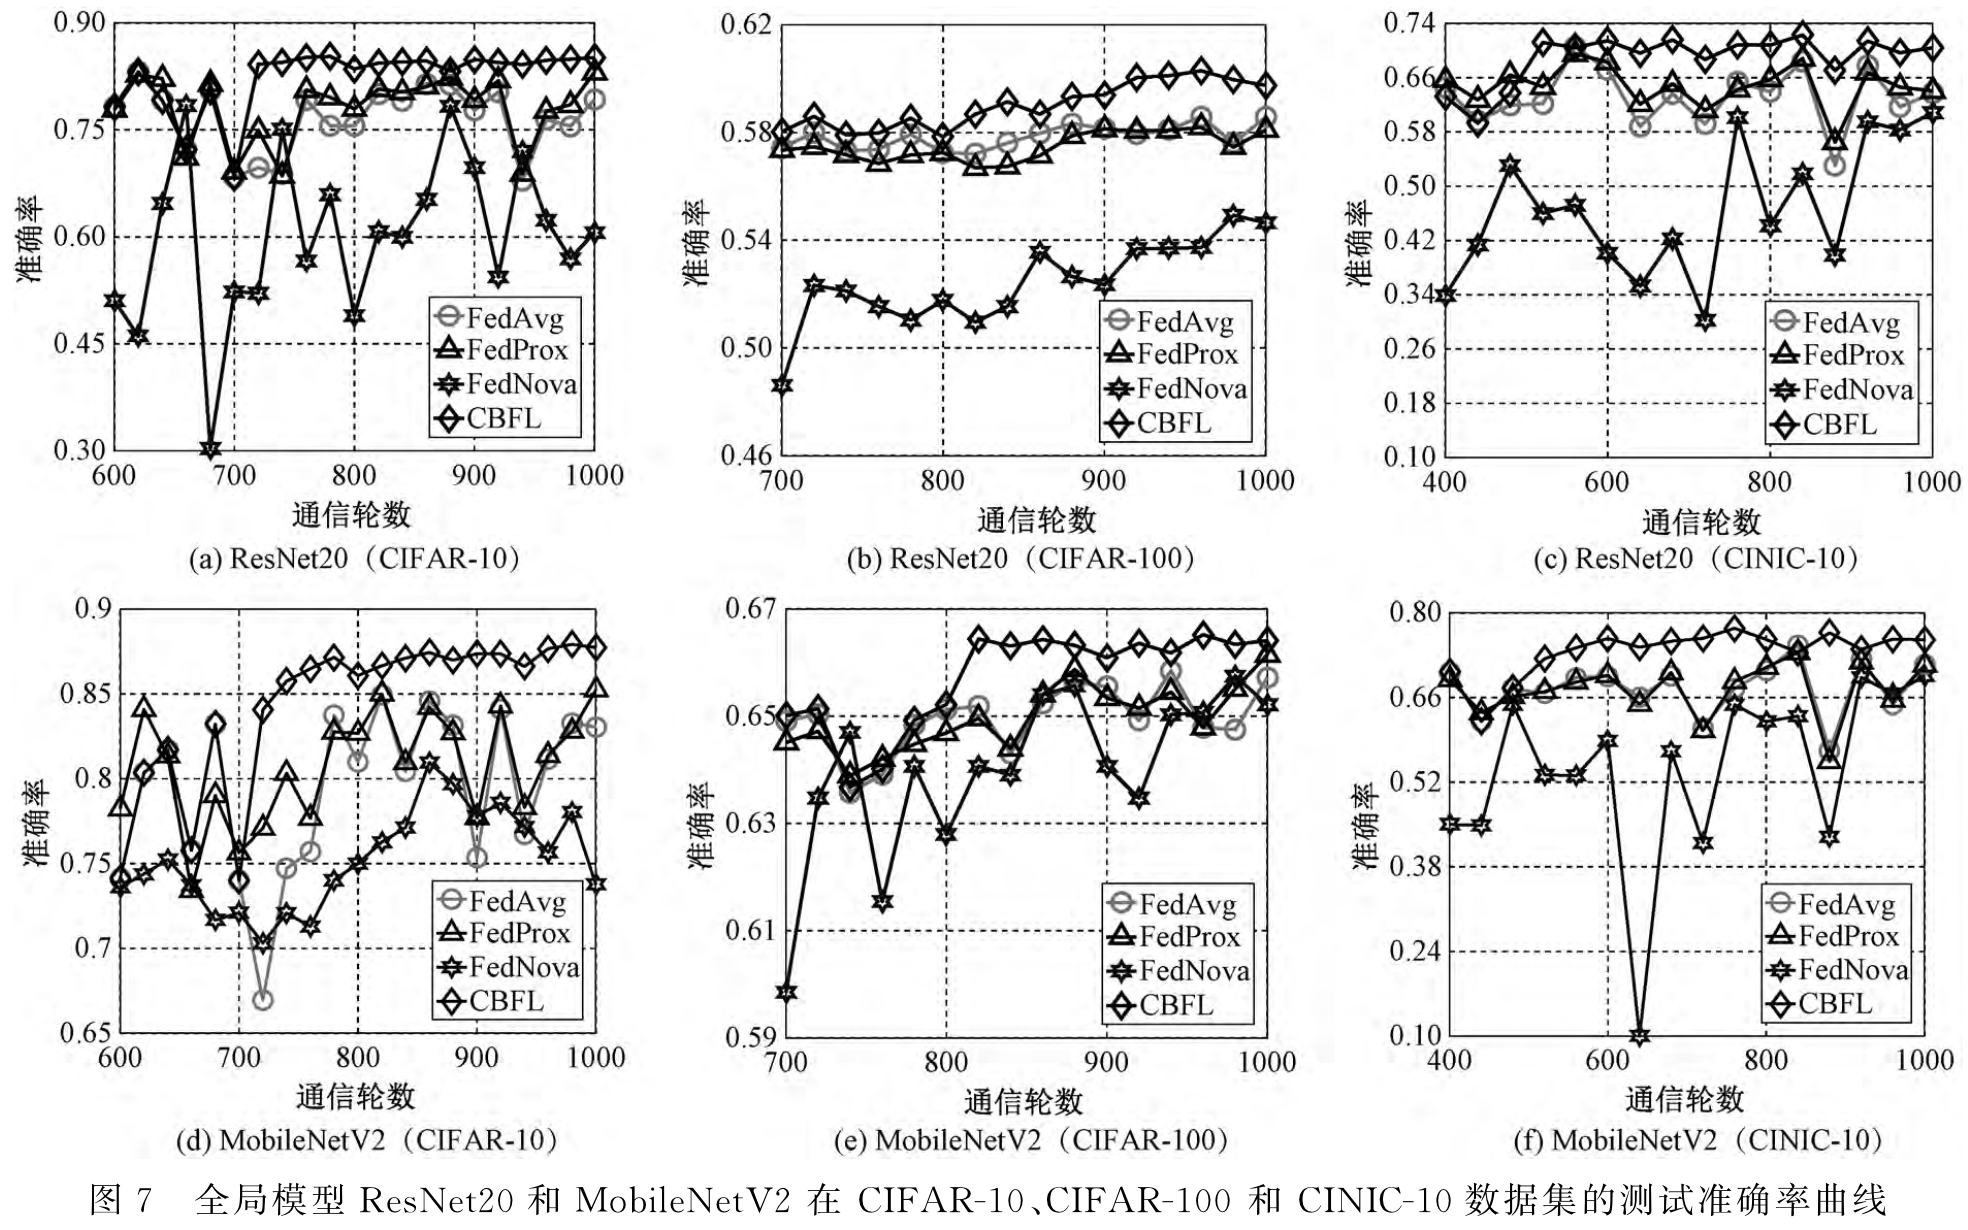
\includegraphics[width=0.75\textwidth]{images/img_expr3}
\end{frame}


\begin{frame}{4.3 实验结果}{Result Analysis}
	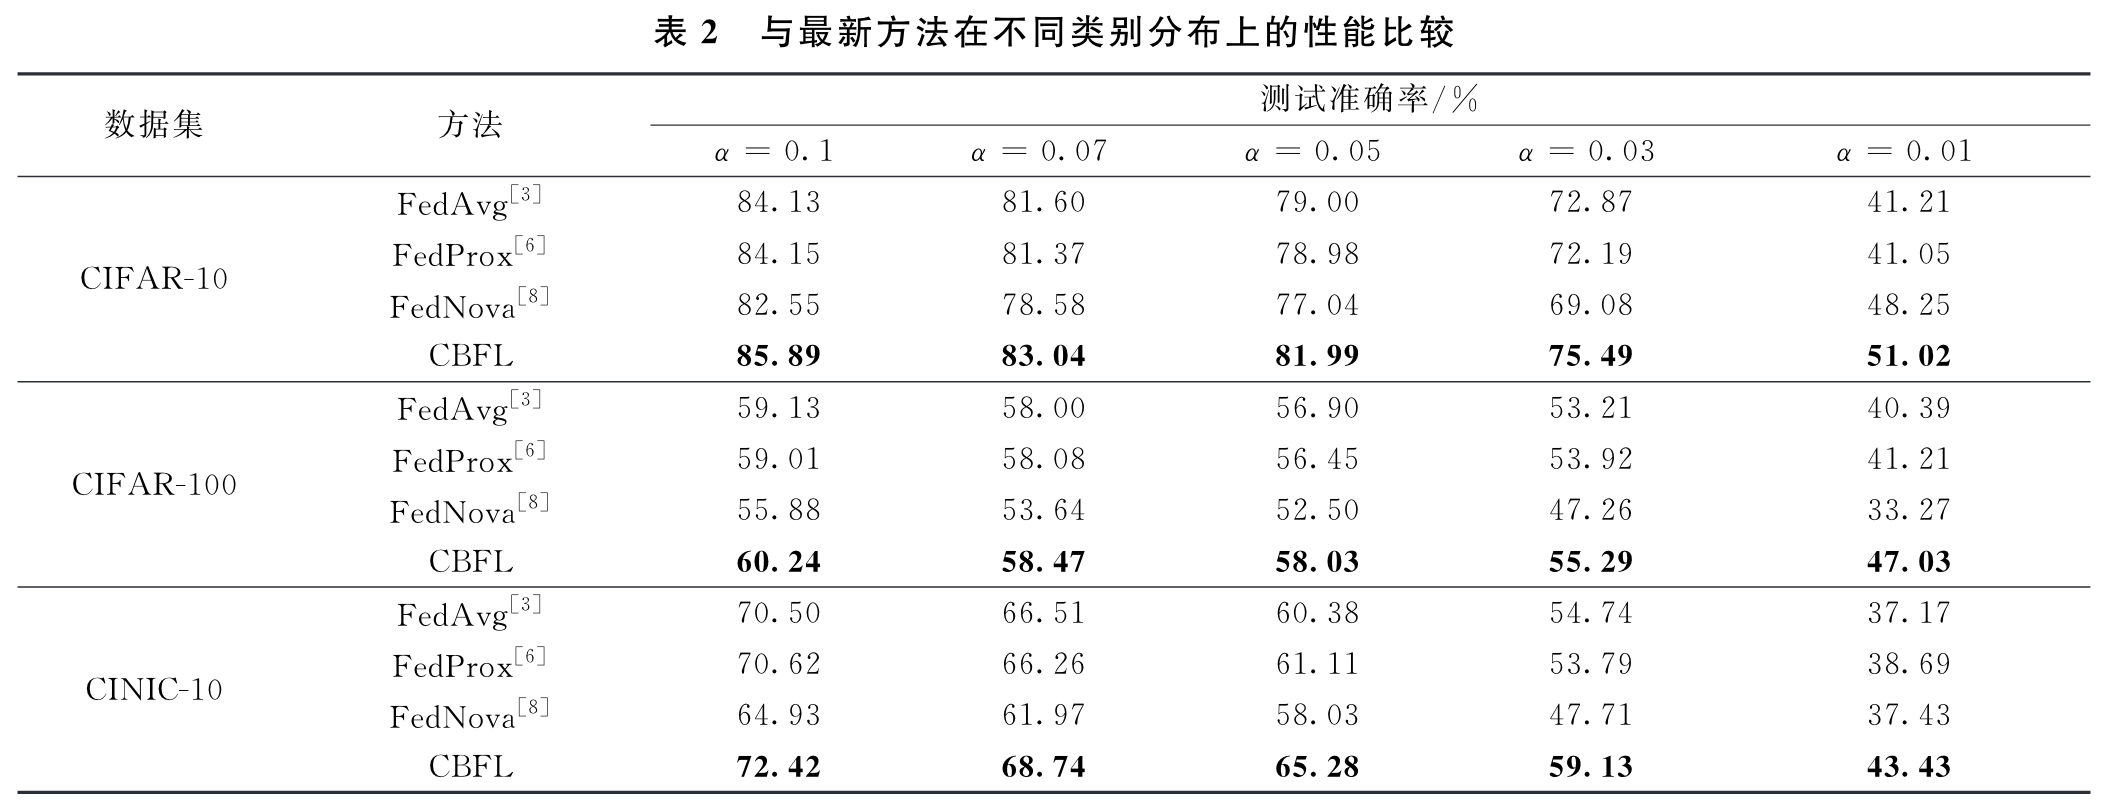
\includegraphics[width=1.\textwidth]{images/img_expr4}
\end{frame}



\section{研究总结}

\begin{frame}{研究总结}

本文提出了一种基于数据生成的类别均衡联邦学习(CBFL)方法.CBFL针对各客户端构造类别均衡的数据集,以降低客户端类别不均衡和客户端之间分布差异的影响.
\\ \hspace*{\fill} \\
具体而言,CBFL设计了一个类别分布均衡器,其由一个类别均衡采样器和一个数据生成器组成.其中,类别均衡采样器以较高概率采样客户端本地数据量不足的类别,然后,数据生成器根据所采样的类别生成相应的虚拟数据.结合本地数据和虚拟数据,客户端构造类别均衡的数据集来进行模型训练,从而有利于构建高性能全局模型.
\end{frame}



\backmatter

\end{document}
